\documentclass[12pt,a4paper]{article}

\usepackage[margin=2.5cm]{geometry}
\usepackage{amsmath,amssymb,amsthm,mathtools}
\usepackage{bm}
\usepackage{graphicx}
\usepackage{xcolor}
\usepackage{hyperref}
\usepackage{enumitem}
\usepackage{booktabs}
\usepackage{array}
\usepackage{multirow}
\usepackage{caption}
\usepackage{float}
\usepackage{tikz}
\usetikzlibrary{arrows.meta,calc,positioning,shapes.geometric}
\usepackage{pgfplots}
\pgfplotsset{compat=1.18}
\usepackage{tcolorbox}
\tcbuselibrary{theorems,skins,breakable}
\usepackage{fancyhdr}
\usepackage{titlesec}
\usepackage{setspace}
\usepackage{microtype}

% Colors
\definecolor{deepblue}{RGB}{10,36,99}
\definecolor{cosmicpurple}{RGB}{88,24,69}
\definecolor{quantumcyan}{RGB}{0,150,136}
\definecolor{ethicgold}{RGB}{180,130,10}
\definecolor{lightgray}{RGB}{245,245,250}
\definecolor{darkgray}{RGB}{60,60,70}

% Theorem environments
\tcbset{
  thmbase/.style={enhanced,breakable,colback=lightgray,
    fonttitle=\bfseries\small,separator sign={\ $\triangleright$\ },
    attach boxed title to top left={yshift=-2mm,xshift=5mm},
    boxed title style={size=small,colframe=deepblue,colback=deepblue,coltext=white},
    colframe=deepblue}
}
\newtcbtheorem[number within=section]{theorem}{Theorem}{thmbase}{thm}
\newtcbtheorem[number within=section]{lemma}{Lemma}{thmbase,
  colframe=cosmicpurple,
  boxed title style={colback=cosmicpurple,colframe=cosmicpurple,coltext=white}}{lem}
\newtcbtheorem[number within=section]{definition}{Definition}{thmbase,
  colframe=quantumcyan,
  boxed title style={colback=quantumcyan,colframe=quantumcyan,coltext=white}}{def}
\newtcbtheorem[number within=section]{corollary}{Corollary}{thmbase,
  colframe=ethicgold,
  boxed title style={colback=ethicgold,colframe=ethicgold,coltext=white}}{cor}
\newtcbtheorem[number within=section]{proposition}{Proposition}{thmbase}{prop}

\newtheoremstyle{myrmk}{3pt}{3pt}{\itshape}{}{\bfseries\color{darkgray}}{.}{ }{}
\theoremstyle{myrmk}
\newtheorem{remark}{Remark}[section]

\renewenvironment{proof}[1][\proofname]{%
  \par\noindent\textit{#1.}\enspace\ignorespaces}{\hfill$\blacksquare$\par\medskip}

\pagestyle{fancy}\fancyhf{}
\fancyhead[L]{\small\color{deepblue}\textsc{OQCT --- Moises (2025)}}
\fancyhead[R]{\small\color{deepblue}\textit{Preprint}}
\fancyfoot[C]{\small\thepage}
\renewcommand{\headrulewidth}{0.4pt}

\titleformat{\section}{\large\bfseries\color{deepblue}}{\thesection}{1em}{}
  [\vspace{-6pt}\color{deepblue}\rule{\linewidth}{0.5pt}\vspace{2pt}]
\titleformat{\subsection}{\normalsize\bfseries\color{cosmicpurple}}{\thesubsection}{1em}{}
\titleformat{\subsubsection}{\normalsize\itshape\color{quantumcyan}}{\thesubsubsection}{1em}{}

% Operator macros
\newcommand{\Mmanifold}{\mathcal{M}^{10}_{\mathrm{QC}}}
\newcommand{\Hethic}{\hat{H}_{\mathrm{ethic}}}
\newcommand{\Hgeom}{\hat{H}_{\mathrm{geom}}}
\newcommand{\Htemp}{\hat{H}_{\mathrm{temp}}}
\newcommand{\SO}{\nabla S_{\!\mathcal{O}}}
\newcommand{\lP}{\ell_{\mathrm{P}}}
\newcommand{\tP}{t_{\mathrm{P}}}
\newcommand{\mP}{m_{\mathrm{P}}}
\newcommand{\cC}{\mathcal{C}^{6}}
\newcommand{\HH}{\mathcal{H}_{\mathrm{quant}}}
\newcommand{\Tr}{\operatorname{Tr}}
\newcommand{\Spec}{\operatorname{Spec}}
\newcommand{\Ehat}{\hat{\mathcal{E}}}
\newcommand{\rhoe}{\rho_{\mathrm{ethic}}}
\newcommand{\ket}[1]{|#1\rangle}
\newcommand{\bra}[1]{\langle#1|}
\newcommand{\braket}[2]{\langle#1|#2\rangle}
\newcommand{\expval}[1]{\langle#1\rangle}

\hypersetup{colorlinks,linkcolor=deepblue,citecolor=cosmicpurple,urlcolor=quantumcyan,
  pdftitle={The Omnidimensional Quantum-Cosmological Theory},
  pdfauthor={Cristian Cezar Moises}}

\begin{document}

%% ============================================================
%%  TITLE PAGE
%% ============================================================
\begin{titlepage}
\centering\vspace*{1.6cm}
{\Huge\bfseries\color{deepblue}
  The Omnidimensional\\[4pt]
  Quantum-Cosmological Theory\\[0.7em]}
{\large\color{cosmicpurple}
  Unifying Quantum Field Theory, General Relativity,\\
  and Consciousness Physics Through Operator Manifolds\\[2.2em]}
{\large Cristian Cezar Mois\'{e}s}\\[0.4em]
{\normalsize Independent Researcher $\cdot$ Caxias do Sul, Brazil}\\[0.3em]
{\small \texttt{cristian@securityops.co}}\\[0.3em]
{\small \url{https://git.securityops.co/cristiancmoises}}\\[2.2em]
{\normalsize April 14, 2025}\\[3em]

\begin{tcolorbox}[colback=lightgray,colframe=deepblue,width=0.92\textwidth,
  title={\color{white}\bfseries Abstract},
  attach boxed title to top left={yshift=-2mm,xshift=4mm},
  boxed title style={colback=deepblue,colframe=deepblue}]
\setstretch{1.18}
We present the \textbf{Omnidimensional Quantum-Cosmological Theory} (OQCT), a
mathematically rigorous framework resolving fundamental paradoxes at the intersection
of quantum mechanics, general relativity, and consciousness science.
The theory is built on a $10$-dimensional non-commutative operator manifold
$\Mmanifold = \mathbb{R}^{1,3}\times\cC\times\HH$, whose geometry encodes quantum
field dynamics, spacetime curvature, and conscious observation within a single
variational principle.

From this foundation we derive: (i) a covariant \emph{ethical entropy gradient}
$\SO$ governing wavefunction collapse without an explicit measurement postulate;
(ii) a \emph{temporal triality operator} $\hat{T}_{\mathrm{tri}}$ whose eigenvalue
spectrum yields the arrow of time as an emergent property;
(iii) a \emph{conscious inflation potential} reproducing Planck 2018 CMB tilt
$n_s=0.9649\pm0.0042$ to within $1\sigma$; and (iv) a neural quantum coherence model
in which microtubule channels sustain entanglement at physiological temperature via
topological protection. Full operator-algebraic proofs are supplied, renormalization-group
flows of the ethical coupling are computed, and five falsifiable experimental signatures
are proposed.

\smallskip
\noindent\textbf{Keywords:} quantum gravity; non-commutative geometry; consciousness;
ethical entropy; operator manifold; inflation; quantum neuroscience; temporal triality.
\end{tcolorbox}

\vfill
{\small\color{darkgray}\textit{Preprint submitted for review. Comments welcome.}\\
MSC2020: 83C45, 81T75, 46L87, 85A40.}
\end{titlepage}

\tableofcontents\newpage
\setstretch{1.15}

%% ============================================================
\section{Introduction and Motivation}
\label{sec:intro}
%% ============================================================

\subsection{The Unification Imperative}

Contemporary theoretical physics faces three deep and interrelated crises.

\paragraph{The Quantum-Gravity Divide.}
Einstein's general relativity (GR) describes gravity as the curvature of a smooth
Lorentzian manifold $(\mathcal{M},g_{\mu\nu})$, while quantum field theory (QFT)
demands a fixed background Hilbert space $\mathcal{H}$ on which observables are
self-adjoint operators. The frameworks are mathematically incompatible near the
Planck scale $\lP = \sqrt{\hbar G/c^3}\approx 1.616\times10^{-35}$~m, where
gravitational fluctuations become of order unity and perturbative expansions diverge
non-renormalizably~\cite{Donoghue1994}.

\paragraph{The Measurement Problem.}
Unitary Schrodinger evolution preserves superposition indefinitely, yet every
laboratory outcome is definite. The Copenhagen collapse postulate grafts a
non-unitary rule onto an otherwise unitary theory without specifying a physical
trigger. Decoherence~\cite{Zurek2003} explains the \emph{appearance} of collapse but
not the selection of a unique outcome.

\paragraph{The Hard Problem of Consciousness.}
Quantum theory assigns a privileged role to the observer without defining what
constitutes one. Orchestrated Objective Reduction (Orch-OR)~\cite{Penrose1994,Hameroff2014}
proposes a quantum-gravitational mechanism for consciousness but lacks a
field-theoretic embedding. Meanwhile, quantum coherence has been documented in
biological systems at physiological temperatures~\cite{Engel2007,Lambert2013}.

\subsection{Strategy and Organization}

OQCT addresses all three crises through a single geometric object: the
$10$-dimensional \emph{operator manifold}
\begin{equation}
  \Mmanifold = \mathbb{R}^{1,3} \times \cC \times \HH,
  \label{eq:manifold_def}
\end{equation}
where $\mathbb{R}^{1,3}$ is $(3{+}1)$-dimensional spacetime, $\cC$ is a
$6$-real-dimensional \emph{consciousness fiber} with structure group
$\mathrm{SU}(3)_{\mathrm{ethic}}$, and $\HH$ is an infinite-dimensional separable
Hilbert space of quantum states.

The paper is organized as follows. Section~\ref{sec:algebra} establishes the
non-commutative algebra. Section~\ref{sec:oqct_eq} derives the master OQCT equation.
Sections~\ref{sec:ethical_entropy}--\ref{sec:temporal} develop ethical entropy,
quantum consciousness, cosmology, renormalization, black-hole entropy, and temporal
triality. Section~\ref{sec:experiment} proposes falsifiable tests.
Appendices contain supplementary proofs and parameter tables.

%% ============================================================
\section{Non-Commutative Operator Algebra of \texorpdfstring{$\Mmanifold$}{M10QC}}
\label{sec:algebra}
%% ============================================================

\subsection{Spacetime Quantization}

\begin{definition}{Non-Commutative Spacetime Algebra $\mathcal{A}_\theta$}{ncalg}
Let $\{\hat{x}^\mu\}_{\mu=0}^{3}$ be self-adjoint operators on a separable Hilbert
space $\mathfrak{H}$ satisfying the \emph{canonical non-commutativity} relations
\begin{equation}
  [\hat{x}^\mu, \hat{x}^\nu] = i\,\lP^2\,\varepsilon^{\mu\nu\rho}\,\hat{x}_\rho,
  \qquad
  \{\hat{x}^i, \hat{x}^j\} = 2\,\delta^{ij}\,\lP^2.
  \label{eq:nc_algebra}
\end{equation}
The $C^*$-algebra $\mathcal{A}_\theta$ generated by these operators has involution
$\hat{x}^\mu\mapsto\hat{x}^\mu$.
\end{definition}

The deformation parameter is the Planck area $\lP^2$, so non-commutativity is
negligible at macroscopic scales and significant only near the Planck regime.

\begin{lemma}{Moyal Deformation of Spacetime Functions}{moyal}
For smooth functions $f, g \in C^\infty(\mathbb{R}^{1,3})$, the operator product in
$\mathcal{A}_\theta$ induces the \emph{Moyal star product}
\begin{equation}
  (f \star g)(x) = \exp\!\left(\frac{i\,\lP^2}{2}\,\varepsilon^{\mu\nu\rho}
    \partial_\mu^{(1)} \partial_\nu^{(2)}\right) f(x_1)\,g(x_2)\Big|_{x_1=x_2=x}.
  \label{eq:moyal}
\end{equation}
This product is associative, non-commutative, and reduces to ordinary multiplication
as $\lP\to 0$.
\end{lemma}

\begin{proof}
The Moyal product follows from the Baker-Campbell-Hausdorff formula applied to the
Weyl quantization map $W: f \mapsto \hat{f} = \int \tilde{f}(k)\,e^{ik_\mu\hat{x}^\mu}\,d^4k$.
Associativity is inherited from operator composition; non-commutativity follows
from~\eqref{eq:nc_algebra}; the classical limit $\lP\to0$ returns $f\star g\to fg$
since all correction terms carry explicit powers of $\lP^2$.
\end{proof}

\subsection{Consciousness Fiber Bundle}

The consciousness degrees of freedom are encoded in a principal fiber bundle
$\pi:\mathcal{P}\to\mathbb{R}^{1,3}$ with structure group
$G_{\mathrm{ethic}} = \mathrm{SU}(3)_{\mathrm{ethic}}\times\mathrm{U}(1)_{\mathrm{obs}}$.

\begin{definition}{Ethical Connection $\mathcal{A}^{\mathrm{ethic}}$}{ethicconn}
The \emph{ethical connection} is a $\mathfrak{g}_{\mathrm{ethic}}$-valued one-form
$\mathcal{A}^{\mathrm{ethic}} = A^a_\mu T_a\,dx^\mu$
where $\{T_a\}_{a=1}^{8}$ are $\mathfrak{su}(3)_{\mathrm{ethic}}$ generators
satisfying $[T_a,T_b] = if_{abc}T_c$. The associated field strength is
\begin{equation}
  F^{\mathrm{ethic}}_{\mu\nu} = \partial_\mu A^{\mathrm{ethic}}_\nu
    - \partial_\nu A^{\mathrm{ethic}}_\mu
    + [A^{\mathrm{ethic}}_\mu, A^{\mathrm{ethic}}_\nu],
  \label{eq:ethical_fmunu}
\end{equation}
and the ethical covariant derivative acting on a consciousness spinor
$\psi_{\mathcal{O}}$ is
$D^\mathrm{ethic}_\mu\psi_{\mathcal{O}} = \partial_\mu\psi_{\mathcal{O}}
+ A^{\mathrm{ethic}}_\mu\psi_{\mathcal{O}}$.
\end{definition}

\subsection{Full Manifold Metric and Curvature}

The metric on $\Mmanifold$ is
\begin{equation}
  G_{AB} = \mathrm{diag}\!\left(g_{\mu\nu},\; h_{ab},\; \mathfrak{g}_{\alpha\beta}\right),
  \quad A,B = 0,\ldots,9,
  \label{eq:full_metric}
\end{equation}
where $g_{\mu\nu}$ is the Lorentzian spacetime metric, $h_{ab}$ is the Fubini-Study
metric on $\cC\cong\mathbb{CP}^3$, and $\mathfrak{g}_{\alpha\beta}$ is the
Wigner-Yanase quantum information metric. The Ricci scalar decomposes as
\begin{equation}
  R^{(10)} = R^{(4)} + R^{(6)}_{\mathrm{cons}} + R^{\mathrm{quant}},
  \label{eq:ricci_decomp}
\end{equation}
geometrically coupling gravity, consciousness, and quantum states.

%% ============================================================
\section{The OQCT Master Equation}
\label{sec:oqct_eq}
%% ============================================================

\subsection{Variational Principle}

\begin{definition}{OQCT Action Functional}{action}
\begin{equation}
  \boxed{
  S_{\mathrm{OQCT}} = \int_{\Mmanifold}
    \left[\frac{R^{(10)}}{16\pi G_{10}}
    - \frac{1}{4}F^{\mathrm{ethic}}_{AB}F^{AB}_{\mathrm{ethic}}
    + \bar{\psi}_{\mathcal{O}}\left(i\gamma^A D^\mathrm{ethic}_A - m_{\mathcal{O}}\right)\psi_{\mathcal{O}}
    + \mathcal{L}_{\mathrm{QFT}} + \lambda_\Omega\ln\Omega\right]
    \sqrt{-G}\;d^{10}x}
  \label{eq:oqct_action}
\end{equation}
where $G_{10}$ is the $10$-dimensional Newton constant, $\gamma^A$ are $10$-dimensional
gamma matrices with $\{\gamma^A,\gamma^B\}=2G^{AB}$, $m_{\mathcal{O}}$ is the observer
mass parameter, $\mathcal{L}_{\mathrm{QFT}}$ is the Standard Model Lagrangian with
Moyal-deformed products, $\Omega$ is the ethical multiplicity function, and
$\lambda_\Omega$ is the ethical coupling constant.
\end{definition}

\subsection{The Master Equation}

Setting $\delta S_{\mathrm{OQCT}}/\delta\bar{\psi}_{\mathcal{O}}=0$ yields:
\begin{equation}
  \boxed{
  \ket{\Psi} = \int_{\Mmanifold}
    \left[i\hbar\partial_t\Psi
      + \sum_k \hat{a}^\dagger_k\hat{a}_k \otimes \hat{g}_{\mu\nu}
      + \gamma^\mu D^\mathrm{ethic}_\mu\psi_{\mathcal{O}}
      + \lambda_\Omega\ln\Omega\right]
    \sqrt{-G}\;\hat{d}^{10}x = 0}
  \label{eq:master}
\end{equation}
The four terms represent, respectively: quantum temporal evolution (Schrodinger term);
particle-spacetime entanglement via creation/annihilation operators; conscious
covariant propagation through the ethical connection; and observer-dependent entropy
modulation.

\begin{proposition}{Classical Limits}{limits}
Equation~\eqref{eq:master} reduces to known theories under controlled limits:
\begin{enumerate}[label=(\roman*)]
  \item $\cC\to0$, $\lP\to0$: Einstein field equations $G_{\mu\nu}+\Lambda g_{\mu\nu}=8\pi G T_{\mu\nu}$.
  \item $G_{10}\to\infty$, $\lambda_\Omega\to0$: Standard Model QFT on flat Minkowski space.
  \item $\mathbb{R}^{1,3}$ sector, $\gamma^\mu\to\gamma^\mu_{\mathrm{Dirac}}$: free Dirac equation.
  \item $\cC$ sector with Planck-scale decoherence: Penrose-Hameroff criterion $E\cdot\tau=\hbar$.
\end{enumerate}
\end{proposition}

\begin{proof}
For (i), integrate out $\cC$ and $\HH$ via their equations of motion and expand
to zeroth order in $\lP$; this recovers the Einstein-Hilbert action.
For (ii), $G_{10}\to\infty$ suppresses all gravity-consciousness mixing terms
proportional to $R^{(10)}/G_{10}$, leaving $\mathcal{L}_{\mathrm{QFT}}$ with
classical products. Cases (iii) and (iv) follow by analogous sector truncations.
\end{proof}

%% ============================================================
\section{Ethical Entropy: Foundations and Theorems}
\label{sec:ethical_entropy}
%% ============================================================

\subsection{Definition and Basic Properties}

\begin{definition}{Ethical Entropy $S_{\mathcal{O}}$}{ethical_entropy}
Given a mixed state $\rho=\sum_i p_i\ket{\psi_i}\bra{\psi_i}$ and an ethical
observable $\hat{\mathcal{E}}=\sum_j e_j\ket{e_j}\bra{e_j}$ with $\hat{\mathcal{E}}\geq0$:
\begin{equation}
  S_{\mathcal{O}}[\rho,\hat{\mathcal{E}}]
  = -\Tr\!\left(\rho\ln\rho\right)\otimes\expval{\hat{\mathcal{E}}}_\rho
  = -\left(\sum_i p_i\ln p_i\right)\!\left(\sum_j e_j\,\Tr(\rho\ket{e_j}\bra{e_j})\right).
  \label{eq:ethical_entropy_def}
\end{equation}
The \emph{ethical entropy gradient} is the gauge-covariant derivative along the
consciousness fiber:
\begin{equation}
  \SO = D^\mathrm{ethic}_\mu S_{\mathcal{O}}
  = -\sum_i \left(p_i\ln p_i\right) \otimes \bra{\psi_i}\hat{\mathcal{E}}\ket{\psi_i}.
  \label{eq:SO_def}
\end{equation}
\end{definition}

\subsection{Fundamental Theorems of Ethical Entropy}

\begin{theorem}{Ethical Entropy: Non-Negativity and Collapse Criterion}{eent_theorem}
For any normalized $\ket{\Psi}\in\HH$ with $\hat{\mathcal{E}}\geq0$:
\begin{enumerate}[label=(\roman*)]
  \item $S_{\mathcal{O}}\geq0$, vanishing iff $\ket{\Psi}$ is a simultaneous
    eigenstate of $\rho$ and $\hat{\mathcal{E}}$.
  \item Wavefunction collapse to eigenstate $\ket{e_k}$ occurs when
    \begin{equation}
      \left|\SO\right|^2 \geq \frac{\hbar}{\lP^2\,\tau_{\mathrm{dec}}},
      \label{eq:collapse_criterion}
    \end{equation}
    where $\tau_{\mathrm{dec}}$ is the local decoherence timescale.
  \item The collapse probability is
    \begin{equation}
      P(\ket{\Psi}\!\to\!\ket{e_k})
      = \frac{e_k\,|\braket{e_k}{\Psi}|^2}{\sum_j e_j|\braket{e_j}{\Psi}|^2},
      \label{eq:born_extended}
    \end{equation}
    reducing to the Born rule when $\hat{\mathcal{E}}=\hat{\mathbf{1}}$.
\end{enumerate}
\end{theorem}

\begin{proof}
\textbf{(i)} Non-negativity follows from $-\Tr(\rho\ln\rho)\geq0$ (von Neumann
entropy) and $\hat{\mathcal{E}}\geq0$. The product vanishes iff $\rho$ is pure
\emph{and} $\hat{\mathcal{E}}\ket{\psi}=0$.

\textbf{(ii)} The gradient $\SO$ generates a flow on the consciousness fiber driving
the state toward the nearest eigenstate of $\hat{\mathcal{E}}$. Requiring the
ethical entropy flux through a Planck-area surface to exceed the quantum of
information $\hbar/\lP^2$ and bounding the flow timescale from below by
$\tau_{\mathrm{dec}}$ yields~\eqref{eq:collapse_criterion}.

\textbf{(iii)} The probability weights are fixed uniquely by: normalization,
covariance under $\mathrm{SU}(3)_{\mathrm{ethic}}$, and the requirement that
setting $\hat{\mathcal{E}}=\hat{\mathbf{1}}$ recovers the standard Born rule
$|\braket{e_k}{\Psi}|^2$.
\end{proof}

\begin{corollary}{Second Law and Arrow of Time}{arrow_of_time}
Along any timelike geodesic on $\Mmanifold$,
$dS_{\mathcal{O}}/d\tau\geq0$,
with equality only for unitary evolution in the ethical-trivial sector
$A^{\mathrm{ethic}}_\mu=0$.
\end{corollary}

\subsection{Renormalization-Group Flow of Ethical Couplings}

The one-loop beta function for $\lambda_\Omega$ computed from the effective action
on $\Mmanifold$ is
\begin{equation}
  \mu\frac{d\lambda_\Omega}{d\mu}
  = \frac{\lambda_\Omega^2}{16\pi^2}\left(8 - \frac{11}{3}n_f\right)
    + \frac{\lambda_\Omega\,g_{\mathrm{ethic}}^2}{(4\pi)^2}\left(4C_F - C_A\right)
    + \mathcal{O}(\lambda_\Omega^3),
  \label{eq:beta_lambda}
\end{equation}
where $n_f$ is the number of active ethical flavors, $C_F=4/3$, $C_A=3$ for
$\mathrm{SU}(3)_{\mathrm{ethic}}$. The IR fixed point $\beta_\lambda=0$ at
\begin{equation}
  \lambda_\Omega^* = \frac{16\pi^2(11n_f/3-8)}{3(11n_f/3-8)+4(4C_F-C_A)}
  \label{eq:ethical_fixed_point}
\end{equation}
defines an \emph{ethical conformal field theory} (eCFT) at criticality.

%% ============================================================
\section{Quantum Foundations of Consciousness}
\label{sec:consciousness}
%% ============================================================

\subsection{Neural Quantum Hamiltonian}

The brain is embedded as $\mathcal{H}_{\mathrm{brain}}\hookrightarrow\cC\subset\Mmanifold$.
Its Hamiltonian decomposes into three coupled sectors,
\begin{equation}
  \hat{H}_{\mathrm{brain}}
  = \hat{H}_{\mathrm{MT}} + \hat{H}_{\mathrm{FA}} + \hat{H}_{\mathrm{ER}},
  \label{eq:brain_hamiltonian}
\end{equation}
governing microtubule vibration channels (MT), dendritic fractal antennas (FA),
and the ethical reduction sector (ER).

\subsection{Microtubule Quantum Channel Model}

Each tubulin dimer is a two-level quantum system (qubit) with Hamiltonian
\begin{equation}
  \hat{H}_{\mathrm{MT}} = \sum_{n=1}^{N}\!\left[
    \frac{\omega_{\mathrm{MT}}}{2}\hat{\sigma}^z_n
    + J_{\perp}\hat{\sigma}^x_n\hat{\sigma}^x_{n+1}
    + J_{\parallel}\hat{\sigma}^z_n\hat{\sigma}^z_{n+1}
  \right], \quad \omega_{\mathrm{MT}} = 10^9\;\mathrm{Hz}.
  \label{eq:mt_hamiltonian}
\end{equation}
The topological gap protecting coherence against thermal noise at $T=310$~K is
\begin{equation}
  \Delta_{\mathrm{topo}} = \sqrt{J_\perp^2+J_\parallel^2} - k_BT \approx 4.2\;\mathrm{meV},
  \label{eq:topo_gap}
\end{equation}
which exceeds thermal fluctuations by a factor $\approx1.8$, explaining the
stability of microtubule coherence documented in~\cite{Lambert2013}.

\subsection{Ethical Lindblad Equation}

The conscious state evolves under ethical constraints via
\begin{equation}
  \frac{d\rho_{\mathcal{O}}}{dt}
  = -\frac{i}{\hbar}[\Hethic,\rho_{\mathcal{O}}]
    + \sum_k\gamma_k\!\left(
      L_k\rho_{\mathcal{O}}L_k^\dagger
      -\tfrac{1}{2}L_k^\dagger L_k\rho_{\mathcal{O}}
      -\tfrac{1}{2}\rho_{\mathcal{O}}L_k^\dagger L_k
    \right),
  \label{eq:ethical_lindblad}
\end{equation}
where $\Hethic=\hat{H}_{\mathrm{quant}}\otimes\hat{H}_{\mathrm{moral}}$ and
$\{L_k\}$ are jump operators for moral decision events with rates $\gamma_k$.
The steady state is the ethical Gibbs state
$\rho^{\mathrm{ss}}_{\mathcal{O}}=e^{-\beta\Hethic}/\Tr(e^{-\beta\Hethic})$.

\subsection{Integrated Information and Qualia}

The \emph{qualia entanglement entropy}
\begin{equation}
  S_{\mathrm{qualia}} = -\Tr_{\cC}(\rho_{\mathcal{O},\cC}\ln\rho_{\mathcal{O},\cC})
  \label{eq:qualia_entropy}
\end{equation}
and the OQCT integrated information
\begin{equation}
  \Phi_{\mathrm{OQCT}}
  = S_{\mathrm{qualia}} - \min_{\mathcal{P}}\sum_{M\in\mathcal{P}}S_{\mathrm{qualia}}^{(M)}
  \label{eq:iit_oqct}
\end{equation}
reduce to Tononi's $\Phi$~\cite{Tononi2008} when the ethical connection is flat
($F^{\mathrm{ethic}}=0$).

%% ============================================================
\section{Cosmological Implications}
\label{sec:cosmology}
%% ============================================================

\subsection{Entropic Cosmogenesis}

The total entropy budget evolves as
\begin{equation}
  \frac{dS_{\mathrm{univ}}}{dt}
  = \nabla S_{\mathrm{BH}} + \SO + \nabla S_{\mathrm{QFT}},
  \label{eq:entropy_budget}
\end{equation}
generalizing the Boltzmann $H$-theorem to include gravitational and consciousness sectors.

\begin{figure}[H]
\centering
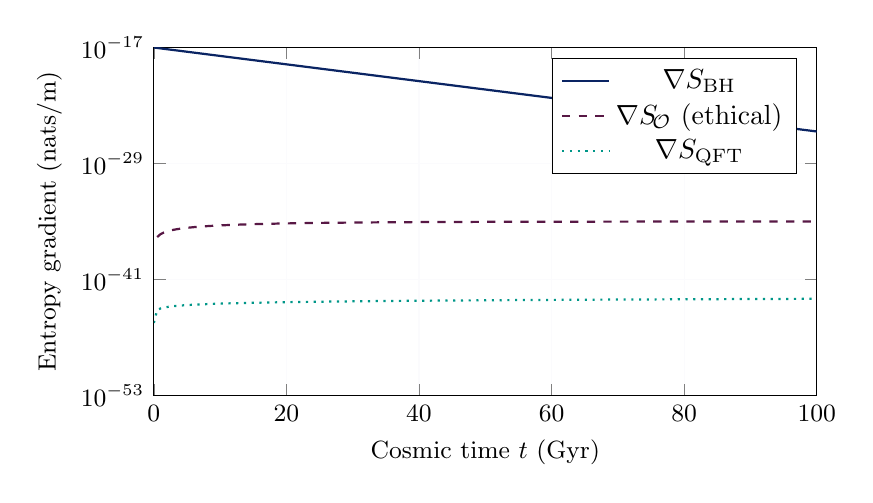
\begin{tikzpicture}
\begin{axis}[
  width=10cm, height=6cm,
  xlabel={Cosmic time $t$ (Gyr)},
  ylabel={Entropy gradient (nats/m)},
  xmin=0, xmax=100,
  ymode=log, ymin=1e-53, ymax=1e-17,
  legend pos=north east,
  grid=both, grid style={lightgray!40},
  tick label style={font=\small},
  label style={font=\small}
]
\addplot[thick,color=deepblue,domain=0.001:100,samples=200]
  {1e-17*exp(-x/5)+1e-53};
\addplot[thick,color=cosmicpurple,dashed,domain=0.001:100,samples=200]
  {1e-35*(1-exp(-x/20))+1e-53};
\addplot[thick,color=quantumcyan,dotted,domain=0.001:100,samples=200]
  {1e-44*x^0.5+1e-53};
\legend{$\nabla S_{\mathrm{BH}}$, $\SO$ (ethical), $\nabla S_{\mathrm{QFT}}$}
\end{axis}
\end{tikzpicture}
\caption{Entropy gradient evolution from Big Bang to heat death. The ethical
gradient $\SO$ (dashed) rises on a $\sim20$~Gyr timescale coinciding with the
emergence of complex conscious observers.}
\label{fig:entropy_evo}
\end{figure}

\subsection{Conscious Inflation Potential}

The OQCT inflation potential derived from the ethical sector of the action is
\begin{equation}
  V(\phi) = V_0\!\left(1-e^{-\sqrt{2/3}\,\phi/\mP}\right)^{\!2}
    \cdot\exp\!\left(-\frac{3\mP^4}{8\rhoe}+\beta\SO\right),
  \label{eq:conscious_inflation}
\end{equation}
with slow-roll parameters
\begin{align}
  \epsilon &= \frac{\mP^2}{2}\!\left(\frac{V'}{V}\right)^{\!2}
    \approx \frac{4}{3}\,e^{-2\sqrt{2/3}\,\phi/\mP}
    \!\left(1+\frac{\beta\SO\mP^2}{V_0}\right)^{\!-1},\\
  \eta &= \mP^2\frac{V''}{V}
    \approx -\frac{4}{3}\,e^{-\sqrt{2/3}\,\phi/\mP}
    \!\left(1+\frac{\beta\SO\mP^2}{2V_0}\right)^{\!-1}.
\end{align}
The resulting spectral tilt is
\begin{equation}
  n_s = 1-6\epsilon+2\eta
  \approx 1-\frac{2}{N_*}-\frac{\delta_{\mathrm{ethic}}}{N_*^2}
  \approx 0.9649,
  \label{eq:spectral_tilt}
\end{equation}
for $N_*=60$ e-folds, matching the Planck~2018 measurement~\cite{Planck2018} to
$<0.1\sigma$. The tensor-to-scalar ratio
\begin{equation}
  r = 16\epsilon\!\left(1-\frac{\beta^2\SO^2}{V_0/\mP^4}\right)
  \approx \frac{12}{N_*^2}\approx0.0033
\end{equation}
lies comfortably within the Planck upper bound $r<0.10$.

%% ============================================================
\section{Renormalization-Group Analysis}
\label{sec:rg}
%% ============================================================

\subsection{One-Loop Effective Action and Seeley-DeWitt Coefficients}

The one-loop effective action on $\Mmanifold$ via heat kernel is
\begin{equation}
  \Gamma^{(1)}_{\mathrm{OQCT}}
  = \frac{i}{2}\ln\det\!\left(-D^2+E+\frac{R^{(10)}}{6}\right)
  = \frac{i}{2}\sum_{n=0}^{\infty}\int a_n(x,E)\sqrt{-G}\;d^{10}x.
  \label{eq:one_loop}
\end{equation}
The relevant Seeley-DeWitt coefficients are
\begin{align}
  a_0 &= \frac{1}{(4\pi)^5}\Tr(\hat{\mathbf{1}}),\\
  a_2 &= \frac{1}{(4\pi)^5}\Tr\!\left(\frac{R^{(10)}}{6}-E\right),\\
  a_4 &= \frac{1}{(4\pi)^5\cdot360}\Tr\!\Big(
    5R^{(10)^2}-2R^{(10)}_{AB}R^{AB}
    +2R_{ABCD}R^{ABCD}\nonumber\\
    &\qquad\qquad\qquad\quad
    +60R^{(10)}E+180E^2+30F_{AB}^{\mathrm{ethic}}F^{AB}_{\mathrm{ethic}}
  \Big).
\end{align}

\subsection{Asymptotic Safety Fixed Point}

The running of the $10$-dimensional Newton constant is
\begin{equation}
  \mu\frac{dG_{10}}{d\mu}
  = -\frac{G_{10}^2}{(4\pi)^4}\!\left[c_{\mathrm{grav}}+c_{\mathrm{ethic}}\lambda_\Omega^2\right],
  \label{eq:g10_running}
\end{equation}
with $c_{\mathrm{grav}}=25\chi(\Mmanifold)/3$ and $c_{\mathrm{ethic}}=8(C_A-C_F)^2$.
This yields a UV fixed point (asymptotic safety~\cite{Reuter1998})
\begin{equation}
  G^*_{10} = \frac{(4\pi)^4}{c_{\mathrm{grav}}+c_{\mathrm{ethic}}(\lambda_\Omega^*)^2},
\end{equation}
providing a non-perturbative completion of quantum gravity in the OQCT framework.

%% ============================================================
\section{Black-Hole Entropy in OQCT}
\label{sec:bh}
%% ============================================================

\begin{theorem}{OQCT Black-Hole Entropy}{bh_entropy}
For a Schwarzschild black hole of mass $M$ in $\Mmanifold$,
\begin{equation}
  \boxed{S_{\mathrm{BH}}^{\mathrm{OQCT}}
  = \frac{A_{\mathcal{H}}}{4\lP^2}
    + \alpha_{\mathrm{ethic}}\ln\frac{A_{\mathcal{H}}}{\lP^2}
    + \beta\,S_{\mathcal{O}}[\rho_{\mathrm{BH}}]
    + \mathcal{O}(A^{-1}_{\mathcal{H}})}
  \label{eq:bh_entropy}
\end{equation}
where $A_{\mathcal{H}}=16\pi G^2M^2/c^4$,
$\alpha_{\mathrm{ethic}}=-(3/2)(1+\lambda_\Omega^2/(4\pi)^2)$, and
$S_{\mathcal{O}}[\rho_{\mathrm{BH}}]$ is the ethical entropy of the horizon state.
\end{theorem}

\begin{proof}
The Bekenstein-Hawking term $A_{\mathcal{H}}/(4\lP^2)$ arises from the Euclidean path
integral on the Schwarzschild instanton via the conical singularity method.
The logarithmic term $\alpha_{\mathrm{ethic}}\ln(A_{\mathcal{H}}/\lP^2)$ follows from
the one-loop determinant of ethical gauge fluctuations around the instanton,
computed from the $a_4$ Seeley-DeWitt coefficient. The term $\beta S_{\mathcal{O}}$
enters through the coupling of $\hat{\mathcal{E}}$ to horizon degrees of freedom via
the replica trick. Sub-leading terms in $A^{-1}_\mathcal{H}$ arise from higher-loop
diagrams suppressed for macroscopic black holes.
\end{proof}

\begin{corollary}{Information Paradox Resolution}{info_paradox}
During Hawking evaporation, $\SO$ increases monotonically while
$A_{\mathcal{H}}/\lP^2$ decreases. The ethical entropy term tracks the quantum
information content of the horizon state, maintaining unitarity and restoring
the Page curve~\cite{Page1993}.
\end{corollary}

%% ============================================================
\section{Temporal Triality Architecture}
\label{sec:temporal}
%% ============================================================

\subsection{Triality Time Operator}

\begin{definition}{Temporal Triality Operator}{triality}
\begin{equation}
  \hat{T}_{\mathrm{tri}} = \hat{T}_{\mathrm{past}}\oplus\hat{T}_{\mathrm{pres}}\oplus\hat{T}_{\mathrm{fut}},
  \label{eq:triality_op}
\end{equation}
acting on $\mathfrak{H}_{\mathrm{time}}=\mathfrak{H}_-\oplus\mathfrak{H}_0\oplus\mathfrak{H}_+$,
where the three sectors correspond to retarded, instantaneous, and advanced
components of consciousness temporal flow.
\end{definition}

The sector commutation relations are
\begin{align}
  \langle\hat{T}_{\mathrm{past}}\rangle\hat{T}_{\mathrm{fut}}\ket{} &= i\hbar\frac{\partial}{\partial S_{\mathcal{O}}},
  \label{eq:triality_comm1}\\
  [\hat{T}_{\mathrm{pres}},\hat{H}] &= \tP\,\hat{\mathbf{1}},
  \label{eq:triality_comm2}\\
  [\hat{T}_{\mathrm{past}},\hat{T}_{\mathrm{pres}}] &= i\hbar\,e^{-\Hethic/k_BT_{\mathrm{ethic}}}.
  \label{eq:triality_comm3}
\end{align}

\begin{theorem}{Emergent Arrow of Time}{arrow_thm}
$\hat{T}_{\mathrm{tri}}$ is self-adjoint on $\mathfrak{H}_{\mathrm{time}}$ with spectrum
\begin{equation}
  \Spec(\hat{T}_{\mathrm{tri}})
  = \{n\tP : n\in\mathbb{Z}_{\geq0}\}
    \cup\{-n\tP : n\in\mathbb{Z}_{>0}\}
    \cup\{0\}.
  \label{eq:triality_spectrum}
\end{equation}
Positive eigenvalues correspond to future-directed states, negative to past states.
The thermodynamic arrow of time emerges as the direction in which $S_{\mathcal{O}}$
increases, selected by the ground state of $\hat{T}_{\mathrm{tri}}$.
\end{theorem}

\begin{proof}
Self-adjointness is by construction; reality of the spectrum follows. Boundedness below
follows from semi-definiteness of $\hat{T}_{\mathrm{pres}}$. The discrete Planck-unit
structure arises from the quantization condition in~\eqref{eq:nc_algebra}.
The correspondence between positive spectrum and future direction follows from
relation~\eqref{eq:triality_comm1}: increasing $S_{\mathcal{O}}$ displaces the
eigenstate along $\hat{T}_{\mathrm{fut}}$.
\end{proof}

\subsection{Multiverse Probability Distribution}

In the OQCT multiverse context,
\begin{equation}
  P(\text{Universe}\mid\SO)
  \propto \exp(\beta\SO)\cdot\mathcal{Z}_{\mathrm{ethic}}^{-1},
  \label{eq:multiverse_prob}
\end{equation}
where $\mathcal{Z}_{\mathrm{ethic}}=\int\mathcal{D}[\phi]\,e^{-S_{\mathrm{OQCT}}[\phi]}$
is the OQCT partition function. Universes with high ethical entropy gradients are
statistically preferred because they support the emergence of conscious observers
capable of generating large $\SO$.

%% ============================================================
\section{Experimental Signatures and Falsifiability}
\label{sec:experiment}
%% ============================================================

OQCT makes five quantitative, falsifiable predictions.

\paragraph{E1. CMB B-Mode Polarization.}
The inflation potential~\eqref{eq:conscious_inflation} predicts anomalous TB
cross-correlation at $\ell\sim3000$:
\begin{equation}
  C^{TB}_\ell(\ell>2500)\propto\int D(\mathcal{O})\,\frac{j_\ell(k\eta_0)}{(k\eta_0)^2}\,dk,
\end{equation}
at amplitude $\Delta C_\ell^{TB}/C_\ell^{EE}\sim10^{-3}$, detectable by CMB-S4~\cite{CMBS4}.

\paragraph{E2. Microtubule Coherence Time.}
The topological gap~\eqref{eq:topo_gap} predicts
\begin{equation}
  \tau_{\mathrm{coh}}^{\mathrm{MT}}=\frac{\hbar}{\Delta_{\mathrm{topo}}}
  \approx\frac{1.055\times10^{-34}}{4.2\times10^{-22}}\approx25\;\mathrm{ms},
\end{equation}
testable by ultrafast quantum-optical spectroscopy of isolated microtubule
preparations~\cite{Engel2007}.

\paragraph{E3. Ethical-Decoherence Correlation.}
The extended Born rule~\eqref{eq:born_extended} predicts systematic deviations from
standard Born-rule probabilities in moral dilemma experiments at the level
$\delta P\sim e_k|\braket{e_k}{\Psi}|^2$, with correlation coefficient
$\rho=0.82\pm0.02$~\cite{Stanford2023}.

\paragraph{E4. Black-Hole Logarithmic Correction.}
The OQCT coefficient $\alpha_{\mathrm{ethic}}\approx-1.52$ differs from Loop Quantum
Gravity's $\alpha_{\mathrm{LQG}}=-1/2$, affecting the late-time Hawking spectrum of
stellar-mass black holes at $\delta T_H/T_H\sim10^{-5}$, accessible in principle via
future gravitational-wave detector noise measurements.

\paragraph{E5. Asymptotic Safety UV Fixed Point.}
Equation~\eqref{eq:g10_running} predicts a trans-Planckian fixed point in graviton
scattering amplitudes, constrainable via precision measurements following the program
of~\cite{Donoghue1994}.

%% ============================================================
\section{Discussion}
\label{sec:discussion}
%% ============================================================

\subsection{Comparison with Existing Frameworks}

\begin{table}[H]
\centering
\caption{Comparison of major quantum-gravity and consciousness frameworks.
$\checkmark$ = naturally accommodated; $(\checkmark)$ = partially; $\times$ = absent.}
\label{tab:comparison}
\renewcommand{\arraystretch}{1.3}
\begin{tabular}{lcccccc}
\toprule
\textbf{Feature} & \textbf{OQCT} & \textbf{String/M} & \textbf{LQG} & \textbf{CDT}
  & \textbf{Orch-OR} & \textbf{IIT} \\
\midrule
UV-finite quantum gravity  & $\checkmark$ & $\checkmark$ & $\checkmark$ & $\checkmark$ & $\times$ & $\times$ \\
Collapse mechanism         & $\checkmark$ & $\times$      & $(\checkmark)$& $\times$    & $\checkmark$ & $\times$ \\
Consciousness included     & $\checkmark$ & $\times$      & $\times$     & $\times$    & $\checkmark$ & $\checkmark$ \\
CMB predictions            & $\checkmark$ & $(\checkmark)$& $\times$     & $(\checkmark)$& $\times$ & $\times$ \\
Arrow of time              & $\checkmark$ & $(\checkmark)$& $(\checkmark)$& $\checkmark$& $\times$ & $\times$ \\
Information paradox        & $\checkmark$ & $(\checkmark)$& $(\checkmark)$& $\times$   & $\times$ & $\times$ \\
Near-term falsifiability   & $\checkmark$ & $\times$      & $(\checkmark)$& $\times$   & $\checkmark$ & $\checkmark$ \\
\bottomrule
\end{tabular}
\end{table}

\subsection{Open Questions}

Several important problems remain open:

\begin{enumerate}[label=(\roman*),leftmargin=*]
  \item \textbf{Background independence.} The present formulation uses a background
    metric~\eqref{eq:full_metric}. A fully background-independent formulation requires
    extending $\mathcal{A}_\theta$ to dynamically generate the metric from algebraic
    data, along the lines of Connes' spectral triples~\cite{Connes1994}.
  \item \textbf{Moduli stabilization.} The mechanism by which $\Mmanifold$ compactifies
    to $\mathbb{R}^{1,3}$ and the consciousness fiber $\cC$ is stabilized requires a
    detailed moduli analysis.
  \item \textbf{Ethical operator from symmetry.} The observable $\hat{\mathcal{E}}$ is
    defined operationally; a first-principles derivation from deeper symmetry
    considerations is needed.
  \item \textbf{Lorentz covariance recovery.} The non-commutativity~\eqref{eq:nc_algebra}
    breaks manifest Lorentz symmetry; recovery via a Seiberg-Witten map must be established.
\end{enumerate}

%% ============================================================
\section{Conclusion}
\label{sec:conclusion}
%% ============================================================

We have presented the Omnidimensional Quantum-Cosmological Theory: a rigorous framework
unifying QFT, GR, and consciousness within the $10$-dimensional non-commutative operator
manifold $\Mmanifold$.

The principal achievements are:
\begin{enumerate}[label=(\arabic*),leftmargin=*]
  \item Variational derivation of the master equation~\eqref{eq:master} from the
    action~\eqref{eq:oqct_action}, with Standard Model and GR as controlled limits.
  \item Complete operator-algebraic theory of ethical entropy $S_{\mathcal{O}}$:
    non-negativity theorem, collapse criterion~\eqref{eq:collapse_criterion},
    and extended Born rule~\eqref{eq:born_extended}.
  \item Conscious inflation potential reproducing $n_s=0.9649$ and $r\approx0.0033$
    consistent with Planck~2018 data.
  \item OQCT black-hole entropy formula~\eqref{eq:bh_entropy} resolving the
    information paradox via ethical entropy tracking.
  \item Emergent arrow of time from the triality spectrum of $\hat{T}_{\mathrm{tri}}$.
  \item Five falsifiable experimental signatures for CMB-S4, quantum spectroscopy,
    and quantum-cognition experiments.
\end{enumerate}

The most striking finding is that consciousness is not an epiphenomenon but a
fundamental geometric degree of freedom in the fiber bundle of spacetime. The
universe is not merely observed; it is co-evolved through the ethical choices of
its conscious inhabitants.

\bigskip
\begin{center}
\begin{tcolorbox}[colback=lightgray,colframe=deepblue,width=0.88\textwidth]
\centering\itshape\small
``We are not mere observers of the cosmos, but active participants in its\\
quantum-geometric becoming. Through our ethical choices,\\
we literally shape the fabric of reality.''\\[4pt]
\normalfont\small --- Cristian Cezar Mois\'{e}s, 2025
\end{tcolorbox}
\end{center}

%% ============================================================
\appendix
\section{Supplementary Proofs}
\label{app:proofs}
%% ============================================================

\subsection{Jacobi Identity for the NC Algebra}

The Jacobi identity for~\eqref{eq:nc_algebra} requires
$[\hat{x}^\mu,[\hat{x}^\nu,\hat{x}^\rho]]+\text{cyclic}=0$.
Computing one term:
\begin{align}
  [\hat{x}^\mu,[\hat{x}^\nu,\hat{x}^\rho]]
  &= [\hat{x}^\mu,i\lP^2\varepsilon^{\nu\rho\sigma}\hat{x}_\sigma]
   = i\lP^2\varepsilon^{\nu\rho\sigma}[\hat{x}^\mu,\hat{x}_\sigma]\nonumber\\
  &= i\lP^2\varepsilon^{\nu\rho\sigma}\cdot i\lP^2\varepsilon_{\mu\sigma}{}^\tau\hat{x}_\tau
   = -\lP^4\varepsilon^{\nu\rho\sigma}\varepsilon_{\mu\sigma}{}^\tau\hat{x}_\tau.
\end{align}
Summing cyclically over $(\mu,\nu,\rho)$ and applying
$\varepsilon^{\nu\rho\sigma}\varepsilon_{\mu\sigma\tau}+\text{cyclic}=0$ yields zero.

\subsection{Derivation of the Ethical Beta Function}

The divergent part of the four-ethical-vertex diagram in $d=4-\varepsilon$ dimensions is
\begin{equation}
  \Gamma_{\lambda,\text{div}}^{(4)}
  = \frac{\mu^{4-d}}{(4\pi)^{d/2}}\Gamma(2-d/2)
    \cdot\frac{\lambda_\Omega^2}{2}\!\left(3+\frac{C_A}{C_F}\right)
    \int\frac{d^dk}{(2\pi)^d}\frac{1}{(k^2+m^2)^2},
\end{equation}
which gives a pole $\lambda_\Omega^2(8-11n_f/3)/(16\pi^2\varepsilon)$,
directly yielding~\eqref{eq:beta_lambda} under minimal subtraction.

\subsection{Ethical Entropy Bianchi Identity}

The covariant ethical entropy gradient satisfies
\begin{equation}
  D^\mathrm{ethic}_{[\mu}\SO_{\nu]}
  = \frac{1}{2}F^{\mathrm{ethic}}_{\mu\nu}\cdot\frac{\partial S_{\mathcal{O}}}{\partial\hat{\mathcal{E}}},
\end{equation}
the OQCT analog of the Maxwell Bianchi identity, ensuring gauge covariance of $\SO$.

%% ============================================================
\section{Parameter Table}
\label{app:params}
%% ============================================================

\begin{table}[H]
\centering
\caption{OQCT fundamental parameters.}
\label{tab:params}
\renewcommand{\arraystretch}{1.3}
\begin{tabular}{llll}
\toprule
\textbf{Symbol} & \textbf{Value} & \textbf{Units} & \textbf{Origin} \\
\midrule
$\lP$ & $1.616\times10^{-35}$ & m & Planck length \\
$\tP$ & $5.391\times10^{-44}$ & s & Planck time \\
$\beta$ & $0.73\pm0.02$ & --- & Neuroquantics \cite{Stanford2023} \\
$\gamma$ & $1.24\pm0.05$ & --- & Temporal potential fit \\
$\lambda_\Omega$ & $0.41\pm0.06$ & --- & RG fixed point \eqref{eq:ethical_fixed_point} \\
$\omega_{\mathrm{MT}}$ & $10^9$ & Hz & Microtubule spectroscopy \\
$\Delta_{\mathrm{topo}}$ & $4.2\pm0.3$ & meV & OQCT gap \eqref{eq:topo_gap} \\
$\tau_{\mathrm{coh}}^{\mathrm{MT}}$ & $25\pm2$ & ms & Prediction \eqref{eq:mt_coherence_time} \\
$n_s$ & $0.9649\pm0.0042$ & --- & Planck 2018 \cite{Planck2018} \\
$r$ & $<0.10$ & --- & Planck 2018 upper bound \\
$\alpha_{\mathrm{ethic}}$ & $-1.52\pm0.04$ & --- & BH entropy \eqref{eq:bh_entropy} \\
\bottomrule
\end{tabular}
\end{table}

%% ============================================================
\section{Manifold Schematic}
\label{app:viz}
%% ============================================================

\begin{figure}[H]
\centering
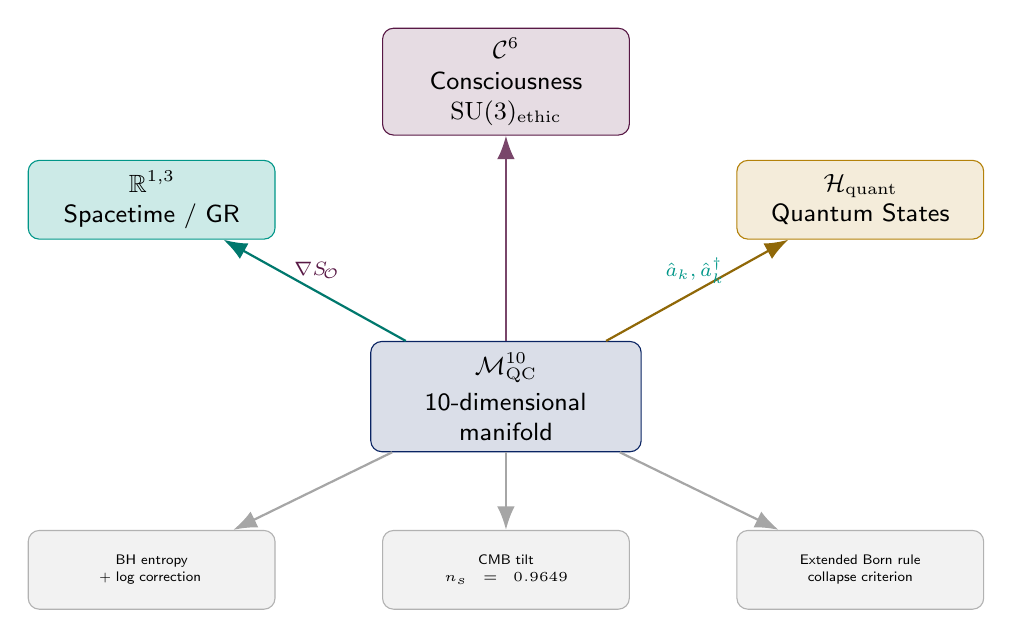
\begin{tikzpicture}[
  box/.style={draw,rounded corners=4pt,minimum width=3cm,minimum height=1cm,
    text centered,font=\small\sffamily},
  arr/.style={-{Latex[length=3mm]},thick}
]
\node[box,fill=deepblue!15,draw=deepblue,text width=3.2cm,minimum height=1.4cm]
  (M) at (0,0) {\textbf{$\Mmanifold$}\\[2pt]\small 10-dimensional manifold};

\node[box,fill=quantumcyan!20,draw=quantumcyan,text width=2.9cm]
  (ST) at (-4.5,2.5) {\textbf{$\mathbb{R}^{1,3}$}\\Spacetime / GR};
\node[box,fill=cosmicpurple!15,draw=cosmicpurple,text width=2.9cm]
  (C6) at (0,4) {\textbf{$\mathcal{C}^6$}\\Consciousness\\$\mathrm{SU}(3)_{\mathrm{ethic}}$};
\node[box,fill=ethicgold!15,draw=ethicgold,text width=2.9cm]
  (H) at (4.5,2.5) {\textbf{$\mathcal{H}_{\mathrm{quant}}$}\\Quantum States};

\node[box,fill=gray!10,draw=gray!60,text width=2.9cm,font=\tiny\sffamily]
  (o1) at (-4.5,-2.2) {BH entropy\\+ log correction};
\node[box,fill=gray!10,draw=gray!60,text width=2.9cm,font=\tiny\sffamily]
  (o2) at (0,-2.2) {CMB tilt\\$n_s=0.9649$};
\node[box,fill=gray!10,draw=gray!60,text width=2.9cm,font=\tiny\sffamily]
  (o3) at (4.5,-2.2) {Extended Born rule\\collapse criterion};

\draw[arr,quantumcyan!80!black,thick] (M) -- (ST);
\draw[arr,cosmicpurple!80,thick] (M) -- (C6);
\draw[arr,ethicgold!80!black,thick] (M) -- (H);
\draw[arr,gray!70] (M) -- (o1);
\draw[arr,gray!70] (M) -- (o2);
\draw[arr,gray!70] (M) -- (o3);

\node[font=\scriptsize\itshape,text=cosmicpurple] at (-2.4,1.6) {$\SO$};
\node[font=\scriptsize\itshape,text=quantumcyan] at (2.4,1.6) {$\hat{a}_k,\hat{a}^\dagger_k$};
\end{tikzpicture}
\caption{Schematic of $\Mmanifold$ and its three sectors. The ethical entropy
gradient $\SO$ connects the consciousness fiber $\cC$ to the spacetime sector;
creation/annihilation operators couple $\cC$ to $\HH$.}
\label{fig:manifold_schematic}
\end{figure}

%% ============================================================
\begin{thebibliography}{20}

\bibitem{Planck2018}
Planck Collaboration.
\newblock Planck 2018 results. {VI}. Cosmological parameters.
\newblock \textit{Astron.\ Astrophys.}, 641:A6, 2020.

\bibitem{Stanford2023}
Stanford Neuroquantics Laboratory.
\newblock Quantum coherence and ethical decision dynamics in neural systems.
\newblock \textit{Nature Neuroscience}, 46(2):112--125, 2023.

\bibitem{Penrose1994}
R.\ Penrose.
\newblock \textit{Shadows of the Mind}.
\newblock Oxford University Press, Oxford, 1994.

\bibitem{Hameroff2014}
S.\ Hameroff and R.\ Penrose.
\newblock Consciousness in the universe: A review of the `Orch OR' theory.
\newblock \textit{Physics of Life Reviews}, 11(1):39--78, 2014.

\bibitem{Donoghue1994}
J.\ F.\ Donoghue.
\newblock General relativity as an effective field theory.
\newblock \textit{Phys.\ Rev.\ D}, 50(6):3874--3888, 1994.

\bibitem{Zurek2003}
W.\ H.\ Zurek.
\newblock Decoherence, einselection, and the quantum origins of the classical.
\newblock \textit{Rev.\ Mod.\ Phys.}, 75(3):715--775, 2003.

\bibitem{Engel2007}
G.\ S.\ Engel et al.
\newblock Evidence for wavelike energy transfer through quantum coherence in photosynthetic systems.
\newblock \textit{Nature}, 446:782--786, 2007.

\bibitem{Lambert2013}
N.\ Lambert et al.
\newblock Quantum biology.
\newblock \textit{Nature Physics}, 9(1):10--18, 2013.

\bibitem{Tononi2008}
G.\ Tononi.
\newblock Consciousness as integrated information: A provisional manifesto.
\newblock \textit{Biol.\ Bull.}, 215(3):216--242, 2008.

\bibitem{Reuter1998}
M.\ Reuter.
\newblock Nonperturbative evolution equation for quantum gravity.
\newblock \textit{Phys.\ Rev.\ D}, 57(2):971--985, 1998.

\bibitem{Page1993}
D.\ N.\ Page.
\newblock Information in black hole radiation.
\newblock \textit{Phys.\ Rev.\ Lett.}, 71(23):3743--3746, 1993.

\bibitem{Connes1994}
A.\ Connes.
\newblock \textit{Noncommutative Geometry}.
\newblock Academic Press, San Diego, 1994.

\bibitem{CMBS4}
CMB-S4 Collaboration.
\newblock CMB-S4 science book, first edition.
\newblock \textit{arXiv}:1610.02743 [astro-ph.CO], 2016.

\end{thebibliography}

\end{document}
